\documentclass[12pt,a4paper,oneside]{book}
\usepackage[utf8]{vietnam}
\usepackage{amsmath, amsfonts, amssymb, graphicx, mathrsfs}
\usepackage{enumerate, boxedminipage, multicol, etoolbox}
\usepackage{tkz-euclide}
\usepackage{tikz-3dplot}
\usepackage{tikz,tkz-tab}
\usetikzlibrary{tikzmark}
\usetikzlibrary{shapes.geometric,arrows,calc,intersections,angles,patterns}
\usetikzlibrary{shadows}
%\usetkzobj{all}
%\usepackage{pgfplots}
%\usepgfplotslibrary{fillbetween}
%\pgfplotsset{compat=1.9}
%\usepackage[top=2cm, bottom=2.5cm, left=1.5cm, right=1.5cm] {geometry}
\usepackage[hidelinks,unicode]{hyperref}
\usepackage{currfile}
%Gói căn lề giấy.
\usepackage[top=2cm, bottom=2cm, left=1.5cm, right=1.5cm]{geometry}

%Xoá thụt đầu dòng.
\setlength\parindent{0pt}
\renewcommand{\baselinestretch}{1.2}


%Gói màu sắc.
%\usepackage[dvipsnames]{xcolor}

%Định nghĩa màu.
\definecolor{mauChuDao}{HTML}{1B3D9F}
\definecolor{cqcqcq}{rgb}{0.75,0.75,0.75}
\definecolor{ocre}{RGB}{24,190,250}
\definecolor{ffqqqq}{rgb}{1.,0.,0.}
\definecolor{qqqqff}{rgb}{0.,0.,1.}
\definecolor{ffffff}{rgb}{1.,1.,1.}
%Gói Tikz.
\usepackage{tikz, tkz-tab, tkz-euclide}
\usetikzlibrary{calc, patterns, shadings, angles, intersections, shapes, quotes, trees}

%Gói ex_test.
%\usepackage[dethi]{ex_test}
% \usepackage[loigiai]{ex_test}
\usepackage[book]{ex_test}
\renewcommand{\loigiaiEX}{{\color{mauChuDao}\faKey~Đáp án}}

%Tạo các môi trường mới.
\usepackage[skins,breakable]{tcolorbox}
\usepackage[explicit,calcwidth]{titlesec}
\usepackage{titletoc}
\usepackage{varwidth}
\tcbuselibrary{raster}
\setcounter{secnumdepth}{4}
\setcounter{tocdepth}{1}

%============================================================%
% CẤU TRÚC SOẠN CHUYÊN ĐỀ HÌNH HỌC
%
% Cách dùng nhanh:
%   \phan{Góc và tia phân giác}
%   \dang{Trung điểm của đoạn thẳng -- đường trung tuyến}
%   \begin{kienthuccanluyen} ... \end{kienthuccanluyen}
%   \begin{vidu} ... \end{vidu}
%   \begin{vidu}[Nâng cao] ... \end{vidu}
%
% Các lệnh dưới đây chỉ lo phần trình bày. Nội dung toán vẫn nhập
% bằng cú pháp LaTeX thông thường, chẳng hạn $AB=10\,\mathrm{cm}$.
%============================================================%
\newcounter{dang}[part]
\renewcommand{\thedang}{\arabic{dang}}
\newcounter{vidu}[dang]
\renewcommand{\thevidu}{\arabic{vidu}}


% Tiêu đề từng dạng; có đánh số, đưa vào mục lục và reset bộ đếm ví dụ.
\newcommand{\dang}[1]{%
	\refstepcounter{dang}%
	\phantomsection%
	\addcontentsline{toc}{section}{PHẦN \thedang. #1}%
	\vspace{0.7\baselineskip}%
	\begin{tcolorbox}[
		enhanced,
		breakable,
		colback=mauChuDao!4,
		colframe=mauChuDao,
		boxrule=0.9pt,
		arc=2mm,
		left=3mm,right=3mm,top=2.2mm,bottom=2.2mm,
		before skip=6pt,after skip=10pt,
		fontupper=\bfseries\fontsize{16}{16}\selectfont,
		borderline west={3pt}{0pt}{mauChuDao}]
		\textcolor{mauChuDao}{PHẦN \thedang. #1}
	\end{tcolorbox}%
	\setcounter{vidu}{0}%
}

% Khối tóm tắt kiến thức/mục tiêu cần luyện.
\newtcolorbox{kienthuccanluyen}[1][]{
	enhanced,
	breakable,
	colback=ocre!7,
	colframe=mauChuDao!75!black,
	boxrule=0.7pt,
	arc=2mm,
	left=4mm,right=4mm,top=2mm,bottom=2mm,
	before skip=6pt,after skip=10pt,
	title={Kiến thức cần luyện},
	fonttitle=\bfseries,
	coltitle=white,
	attach boxed title to top left={xshift=4mm,yshift*=-\tcboxedtitleheight/2},
	boxed title style={colback=mauChuDao,colframe=mauChuDao,arc=1.5mm},
	#1
}

% Ví dụ tự đánh số theo từng dạng. Tham số tùy chọn dùng cho nhãn
% như [Nâng cao], [Cơ bản], [Có hình vẽ], ...
\newenvironment{vidu}[1][]{%
	\refstepcounter{vidu}%
	\def\nhanvidu{#1}%
	\begin{tcolorbox}[
		enhanced,
		breakable,
		colback=white,
		colframe=mauChuDao!65,
		boxrule=0.7pt,
		arc=1.5mm,
		left=4mm,right=4mm,top=2mm,bottom=2mm,
		before skip=7pt,after skip=9pt,
		title={Ví dụ \thevidu\ifx\nhanvidu\empty\else\ -- \nhanvidu\fi},
		fonttitle=\bfseries,
		coltitle=mauChuDao,
		colbacktitle=mauChuDao!8,
		boxed title style={boxrule=0pt,arc=0pt}]
}{%
	\end{tcolorbox}%
}

% Hai khối phụ để ghi nhận xét phương pháp và điều cần nhớ.
\newtcolorbox{nhanxet}[1][]{
	breakable,
	colback=black!2,
	colframe=black!35,
	boxrule=0.5pt,
	arc=1.5mm,
	title={Nhận xét},
	fonttitle=\bfseries,
	#1
}
\newtcolorbox{ghinho}[1][]{
	breakable,
	colback=yellow!8,
	colframe=orange!70!black,
	boxrule=0.6pt,
	arc=1.5mm,
	title={Ghi nhớ},
	fonttitle=\bfseries,
	#1
}

%========= Công thức toán =========%
\everymath{\displaystyle}
%Dấu hệ hoặc.
\newcommand{\hoac}[1]
{
	\left[\begin{aligned}#1\end{aligned}\right.
}
%Dấu hệ và.
\newcommand{\heva}[1]
{
	\left\{\begin{aligned}#1\end{aligned}\right.
}
%==================================%

%=======Tùy biến môi trường =======%
\makeatletter
%Tùy chỉnh Mục lục
\usepackage{ifoddpage}
\titleformat{name=\chapter,numberless}[display]
{\normalfont\huge\bfseries}
{}
{-1cm}
{%
	\begin{tikzpicture}[remember picture, overlay]%
		\draw[fill=mauChuDao, rounded corners=15pt] (12.5,-.75) rectangle (20,1.3);%
		\draw (13.5,0.2) node [right]{\color{white}\fontsize{25pt}{1pt}\fontfamily{qag}\selectfont\bfseries\MakeUppercase{#1}};%
	\end{tikzpicture}
}
[
\vspace{1cm}
]

\renewcommand*\l@part[2]{%
	\ifnum \c@tocdepth >-2\relax
	\addpenalty{-\@highpenalty}%
	\addvspace{2.25em \@plus\p@}%
	\setlength\@tempdima{3em}%
	\begingroup
	\parindent \z@ \rightskip \@pnumwidth
	\parfillskip -\@pnumwidth
	{\leavevmode
		\large \bfseries PHẦN #1\dotfill
		\hb@xt@\@pnumwidth{\hss #2%
			\kern-\p@\kern\p@}}\par
	\nobreak
	\global\@nobreaktrue
	\everypar{\global\@nobreakfalse\everypar{}}%
	\endgroup
	\fi}
%Title chapter
\renewcommand*\l@chapter[2]{%
	\ifnum \c@tocdepth >\m@ne
	\addpenalty{-\@highpenalty}%
	\vskip 1.0em \@plus\p@
	\setlength\@tempdima{1.5em}%
	\begingroup
	\parindent \z@ \rightskip \@pnumwidth
	\parfillskip -\@pnumwidth
	\leavevmode \bfseries
	\advance\leftskip\@tempdima
	\hskip -\leftskip
	\hspace*{0.5cm}CHƯƠNG #1\nobreak\dotfill
	\nobreak\hb@xt@\@pnumwidth{\hss #2%
		\kern-\p@\kern\p@}\par
	\penalty\@highpenalty
	\endgroup
	\fi}
%Title section
\renewcommand*\l@section[2]{%
	\ifnum \c@tocdepth >\m@ne
	\addpenalty{-\@highpenalty}%
	\vskip 0.5em \@plus\p@
	\setlength\@tempdima{1.5em}%
	\begingroup
	\parindent \z@ \rightskip \@pnumwidth
	\parfillskip -\@pnumwidth
	\leavevmode \bfseries
	\advance\leftskip\@tempdima
	\hskip -\leftskip
	\hspace*{1cm}#1\nobreak\dotfill
	\nobreak\hb@xt@\@pnumwidth{\hss #2%
		\kern-\p@\kern\p@}\par
	\penalty\@highpenalty
	\endgroup
	\fi}

%----------------------------------%
%Môi trường Phần
\renewcommand{\thepart}{\Roman{part}}
\titleformat{\part}
{
	\thispagestyle{fancy}\filcenter\color{mauChuDao}\bfseries
}
{		
	\definecolor{mauPhan}{HTML}{FF0066}
	
\begin{tikzpicture}
		\node at (0,0){\fontsize{28pt}{1pt}\selectfont\MakeUppercase\partname};
		\node[shape = star, fill =mauChuDao, inner sep = 5pt] at (0,0)[shift = {(0,-4)}] {\textcolor{white}{\fontsize{70pt}{1pt}\selectfont \thepart}};
	\end{tikzpicture}
}
{0 cm}
{
	\vskip 5pt\titlerule[2.5pt]\vskip 1.5pt\titlerule[1pt]\vskip 5pt 
	\fontsize{25pt}{10pt}\selectfont\MakeUppercase{#1}
}
%----------------------------------%
%Môi trường Chương
\renewcommand{\chapter}
{
	\if@openright\cleardoublepage\else\clearpage\fi
	\global\@topnum\z@
	\@afterindentfalse
	\secdef\@chapter\@schapter
}
\titleformat{\chapter}
{}
{}
{0em}
{
	\begin{tikzpicture}
		\node (base){\color{mauChuDao}\bfseries\fontsize{18}{0}\selectfont \faGripfire CHƯƠNG\faGripfire};
		\node[draw=mauChuDao,circle,line width=2pt] (num) at ([yshift=-0.9cm]base.-90){\color{mauChuDao}\fontsize{30}{0}\selectfont\thechapter};
		\node at ([yshift=-0.3cm]num.-90){\color{mauChuDao}\faGg\faGg\faGg};
		\draw[double, double distance=0.1cm, line width=2pt, mauChuDao] ([shift={(1.8,-0.5)}]num.south east)--++(\textwidth-5cm,0);
		\node[text width={\textwidth - 5cm}, right] (content) at ([shift={(1.3,0)}]num.0){\color{mauChuDao}\bfseries\fontsize{15pt}{0pt}\selectfont\MakeUppercase{#1}};
	\end{tikzpicture}
}
[   
\setcounter{dn}{0}
\setcounter{dl}{0}
\setcounter{hq}{0}
]
\titlespacing{\chapter}{0cm}{0cm}{0.5cm}[0cm]
%----------------------------------%
%Môi trường Bài
\renewcommand*{\thesection}{\arabic{section}}
\titleformat{\section}
{\centering}
{}
{0pt}
{
	\begin{tikzpicture}
		\node[text width={\textwidth-2cm},text centered] (A){
			\color{mauChuDao}\bfseries\fontsize{15}{0}\selectfont\S\thesection. \MakeUppercase{#1}
		};
	\end{tikzpicture}
}
\titlespacing{\section}{0cm}{1cm}{0cm}[0cm]

%----------------------------------%
%Môi trường Mục
\renewcommand*{\thesubsection}{\Alph{subsection}}
\titleformat{\subsection}
{
	\bfseries
}
{
	\begin{tikzpicture}
		\node[mauChuDao, shape=star, draw, line width = 1pt, inner sep=2pt] (char){\fontsize{15}{0}\selectfont\color{mauChuDao}\bfseries\thesubsection};
		\node[right, text width=\textwidth-2cm] (content) at ([xshift=0.5cm]char.0){\fontsize{13}{0}\selectfont\color{mauChuDao}\bfseries\MakeUppercase{#1}};
	\end{tikzpicture}
}
{0pt}
{}
[
]
\titlespacing{\subsection}{-0.4cm}{0cm}{0cm}[0cm]
%----------------------------------%
%Môi trường mục con.
\renewcommand*{\thesubsubsection}{\arabic{subsubsection}}
\titleformat{\subsubsection}
{
	\bfseries
}
{
	\begin{tikzpicture}
		\node[mauChuDao, shape=circle, draw, fill=mauChuDao, line width = 1pt, inner sep=2pt] (char){\fontsize{12}{0}\selectfont\color{white}\bfseries\thesubsubsection};
		\node[right=0.5cm, text width=\textwidth-2cm] (content) at (char.0){\fontsize{12}{0}\selectfont\color{mauChuDao}\bfseries\MakeUppercase{#1}};
	\end{tikzpicture}
}
{0pt}
{}
[
]
\titlespacing{\subsubsection}{-0.15cm}{0cm}{0cm}[0cm]


%Môi trường Bài tập
\newtheorem{bt}{\bfseries Bài}
%Môi trường Chứng minh.
\theoremstyle{nonumberplain} 
\theoremheaderfont{\bfseries\slshape} 
\theorembodyfont{\normalfont}
\theoremsymbol{\ensuremath{_\blacksquare}} 
\newtheorem{proof}{Chứng minh}
\newcommand{\chm}[1]{\begin{proof}#1\end{proof}}
%----------------------------------%
\makeatother
%==================================%


%==================================%
\newcommand{\tikzHeaderFooter}{
	\begin{tikzpicture}[scale=1, font=\footnotesize, line join=round, line cap=round,>=stealth, overlay, remember picture]
		\def\h{1} %Chiều cao của box
		\coordinate (D) at (current page.east);
		\coordinate (T) at (current page.west);
		\coordinate (B) at (current page.north);
		\coordinate (N) at (current page.south);
		\coordinate (TN) at (current page.south west);
		\coordinate (DN) at (current page.south east);
		\coordinate (TB) at (current page.north west);
		\coordinate (DB) at (current page.north east);
		\coordinate (CT) at (current page.center);
		\fill[mauChuDao] (TB)++(\paperwidth*0.42,-0.5)--++(180:\paperwidth*0.42)--++(-90:\h)--++(0:\paperwidth*0.37)arc(-90:-45:10pt)
		(DB)++(-\paperwidth*0.1,-\h-0.5)--++(0:\paperwidth*0.1)--++(90:\h)--++(180:\paperwidth*0.05) arc (90:135:10pt)
		(TN)++(\paperwidth*0.7,0.5)--++(180:\paperwidth*0.7)--++(90:\h)--++(0:\paperwidth*0.65) arc (90:45:10pt)
		
		;
		\draw[mauChuDao, line width=4pt] (DN)++(0,0.5)--++(180:\paperwidth);
		\draw[mauChuDao, -o, line width=2pt](DB)++(0,-\h-0.5)--++(180:\paperwidth*0.55)
		;
		%		\fill[mauChuDao] (TB)--++(-90:\paperheight/12)..controls +(45:2)..($(DB)+(-90:\paperheight/24)$)--(DB) (DN)--++(90:\paperheight/12)..controls +(225:2)..($(TN)+(90:\paperheight/24)$)--(TN);node[mauChuDao, right]{\bfseries STAR EDUCATION}
		\draw ($(TB)+(-90:1)+(0:0.5)$) node[right]{\facebook};
		\draw ($(DB)+(-90:1)+(180:2)$) node[left]{\hotline};
		\draw ($(DN)+(90:0.95)+(180:1.5)$) node[left]{\sotrang};
		\draw ($(TN)+(90:0.95)+(0:1)$) node[right]{\diachi};
		\path (CT) node[opacity=0.9]{
			
\includegraphics[scale=1]{logo/Logo.png}
		};
	\end{tikzpicture}
}

%Tạo liên kết facebook.
\newcommand{\facebook}{
	\definecolor{mauFabeook}{HTML}{61C1F2}
	\href{https://www.facebook.com/hocthemstar}{
		\tikz{
			\node (A){\fontsize{30}{0}\selectfont};
			\draw(A.10)node[right=0.2em]{\fontsize{15}{0}\selectfont~\textsf{\color{white} \textbf{\textit{STAR EDUCATION}}}};
		}
	}
}

%Tạo số điện thoại.
\newcommand{\hotline}{
	\definecolor{mauHotLine}{HTML}{DE0000}
	\fontsize{15}{0}\selectfont{\bfseries\color{mauChuDao}\faIcon{mobile-alt}}~\hspace{0.2cm}\color{mauChuDao}\textbf{089 66 888 30 - 089 66 888 40}}

%Tạo đếm số trang.
\newcommand{\sotrang}{\fontsize{15}{0}\selectfont\color{mauChuDao}\textbf{Trang \thepage/\pageref{LastPage}}}

%Tạo câu châm ngôn.
\newcommand{\chamngon}{\fontsize{15}{0}\selectfont\color{white}\textbf{\textit{Sẽ Không Làm Được Nếu Không Làm}}}

%Tạo địa chỉ
\newcommand{\diachi}{\fontsize{13}{0}\selectfont{\color{white} \faIcon{map-marker-alt}}\color{white}\textbf{ 16/2 Trần Thiện Chánh, P.12, Q.10, TP.HCM}}
\usepackage{fancyhdr}
%\usepackage[unicode,bookmarksopen=true,psdextra,plainpages=false,pdfpagelabels=true, hidelinks]{hyperref}
\usepackage{bookmark}
\usepackage{lastpage, fontawesome5}
\pagestyle{fancy}
\setlength{\headheight}{15pt}
\rhead{}
\chead{\tikzHeaderFooter}
\lhead{}
\rfoot{}
\cfoot{}
\lfoot{}
\renewcommand{\headrulewidth}{0pt}
\renewcommand{\footrulewidth}{0pt}


%Gói khác
\usepackage{diagbox, longtable}
%Điều chỉnh tabular
\renewcommand{\arraystretch}{1.2}
\renewcommand{\arrayrulewidth}{1pt}
%Chỉnh lại khoãng cách dòng trong Ex_test
\renewcommand{\dotlineEX}[1]{
	\def\numlinedot{#1}
	\par
	\foreach \dotline in{1,...,\numlinedot}
	{	
		\noindent\dotfill\\[0.3cm]
		\par
	}
}

\newcommand{\dotlineansVD}[1]{
	\renewcommand{\FalseEX}{\stepcounter{dapan}{\textbf{\Alph{dapan}}}.}
	\renewcommand{\TrueEX}{\stepcounter{dapan}{\textbf{\Alph{dapan}}}.}
	\def\True{\setcounter{numTrue}{\thedapan}\setcounter{numTrueSol}{\thedapan}} 
	\AtBeginEnvironment{vd}{%
		\renewcommand{\loigiai}[1]{%
			\endboxVD
			\par\noindent\textbf{\loigiaiEX }
			\dotlineEX{#1}
			\def\endboxVD{}
		}
	}
}
\newcommand{\soso}{\mathbin{/\mkern-6mu/}}


\usepackage{enumitem}
\setlist[enumerate,1]{label={\alph*)}}
\makeatletter
\newenvironment{vdcases}[1][l]{%
	\let\@ifnextchar\new@ifnextchar
	\left\lbrace
	\def\arraystretch{1.2}%
	\array{@{}#1@{\quad}l@{}}
}{%
	\endarray\right.
}
\makeatother

\usepackage{utfsym}


\begin{document}
	\thispagestyle{empty}
	\begin{tikzpicture}[remember picture,overlay]
		\node[align=center,font= \bfseries] at (current page.center) {
			\textsf{\large STAR EDUCATION}\\\\			
			\textsf{\huge ÔN TẬP HÌNH HỌC}\\
			\textsf{\Huge LỚP 7TC3} \\ \\
			\Large Năm học: 2026 -- 2027		
		};
		\node[
			align=center,
			font=\large
		] at ([yshift=2.5cm]current page.south) {
			Biên soạn:\\[4pt]
			\textbf{HOÀNG YẾN TRANG}
		};
	\end{tikzpicture}

	\setcounter{page}{1}

	\newpage
    \dang{GÓC Ở VỊ TRÍ ĐẶC BIỆT - TIA PHÂN GIÁC CỦA MỘT GÓC - HAI ĐƯỜNG THẲNG VUÔNG GÓC}
	\subsection{Dạng 1. Tính số đo góc}
\noindent

\begin{bt}
	Trên đường thẳng $xy$ lấy điểm $O$.
	Trên cùng một nửa mặt phẳng có bờ là đường thẳng $xy$, vẽ hai tia $Om$ và $On$ sao cho
	hai góc $\widehat{xOm}$ và $\widehat{yOn}$ là hai góc phụ nhau và
	$\widehat{xOm}=56^\circ$.
	
	\begin{enumerate}[label=\alph*)]
		\item Tính góc $\widehat{yOn}$.
		
		\item Tính góc kề bù với góc $\widehat{xOm}$.
		
		\item Tính góc kề bù với góc $\widehat{yOn}$.
		
		\item Vẽ tia $Ot$ là tia phân giác của góc $\widehat{mOn}$.
		Tính số đo góc $\widehat{tOy}$.
	\end{enumerate}
\end{bt}

\begin{bt}
	Cho $\widehat{AOB}$ và $\widehat{BOC}$ là hai góc kề bù. Biết
	$\widehat{BOC}=5\widehat{AOB}$.
	
	\begin{enumerate}[label=\alph*)]
		\item Tính số đo mỗi góc.
		\item Gọi $OD$ là tia phân giác của $\widehat{BOC}$. Tính số đo $\widehat{AOD}$.
	\end{enumerate}
\end{bt}


\subsection{Dạng 2. Chứng minh một tia là tia phân giác}
\noindent
\begin{bt}
	Trên cùng một nửa mặt phẳng có bờ chứa tia $Ox$, vẽ hai tia $Oy$ và $Ot$
	sao cho $\widehat{xOy}=30^\circ$ và $\widehat{xOt}=60^\circ$.
	
	\begin{enumerate}[label=\alph*)]
		\item Chứng minh tia $Oy$ nằm giữa hai tia $Ox$ và $Ot$.
		
		\item Tính số đo $\widehat{yOt}$. Từ đó chứng minh $Oy$ là tia phân giác
		của $\widehat{xOt}$.
		
		\item Gọi $Om$ là tia đối của tia $Ox$ và $Oz$ là tia phân giác của
		$\widehat{mOt}$. Tính số đo $\widehat{tOz}$.
		
		\item Chứng minh $Ot$ là tia phân giác của $\widehat{xOz}$.
	\end{enumerate}
\end{bt}
\begin{bt}
	Cho $\widehat{xOy}=120^\circ$. Bên trong $\widehat{xOy}$, vẽ tia $Om$
	sao cho $\widehat{yOm}=30^\circ$ và vẽ tia $On$ sao cho
	$\widehat{yOn}=90^\circ$.
	
	\begin{enumerate}[label=\alph*)]
		\item So sánh số đo $\widehat{xOn}$ và $\widehat{yOm}$.
		
		\item Gọi $Ot$ là tia phân giác của $\widehat{xOy}$. Chứng minh rằng
		$Ot$ cũng là tia phân giác của $\widehat{mOn}$.
	\end{enumerate}
\end{bt}
\newpage
\noindent
\subsection{Dạng 3. Hai tia đối nhau -- hai góc đối đỉnh}
\begin{ghinho}
	\textbf{Nếu đề không chỉ rõ đó là hai góc đối đỉnh thì
	\textcolor{red!75!black}{phải giải thích} trước khi sử dụng.}
\end{ghinho}

\begin{bt}
	Cho góc bẹt $\widehat{xOy}$. Trên cùng một nửa mặt phẳng có bờ là đường
	thẳng $xy$, vẽ hai tia $Ot$, $Oz$; trên nửa mặt phẳng đối diện, vẽ tia
	$Oh$ sao cho $\widehat{xOz}=\widehat{yOt}=\widehat{xOh}=50^\circ.$
	Hai góc $\widehat{xOh}$ và $\widehat{yOt}$ có phải là hai góc đối đỉnh
	không? Vì sao?

\begingroup
	\bfseries\itshape\boldmath
	Gợi ý: Dùng tính chất bắc cầu để chứng minh
	\[
		\begin{aligned}
			a+b &= 180^\circ\\
			c+b &= 180^\circ
		\end{aligned}
		\quad\Longrightarrow\quad a=c.
	\]
\endgroup
\end{bt}

\begin{bt}
	Cho hai đường thẳng $xy$ và $x'y'$ cắt nhau tại $O$. Vẽ tia $Oz$ là
	tia phân giác của $\widehat{x'Oy}$ và tia $Ot$ là tia phân giác của
	$\widehat{xOy'}$.
	
	\begin{enumerate}[label=\alph*)]
		\item Chứng minh $\widehat{xOt}=\widehat{x'Oz}$.
		
		\item Chứng minh $\widehat{xOt}$ và $\widehat{yOz}$ là hai góc đối đỉnh.
	\end{enumerate}
\end{bt}

\begin{bt}
	Cho hai đường thẳng $a$ và $b$ cắt nhau tại $O$, tạo thành bốn góc
	$\widehat{O_1}$, $\widehat{O_2}$, $\widehat{O_3}$, $\widehat{O_4}$
	như hình dưới đây. Tính số đo các góc trong mỗi trường hợp sau:

	\begin{flushright}
		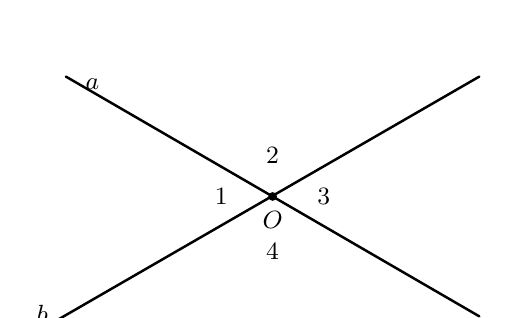
\begin{tikzpicture}[
			scale=1.05,
			line cap=round,
			line join=round,
			font=\small
		]
			\coordinate (O) at (0,0);

			% Hai đường thẳng a và b
			\draw[line width=0.9pt] (-2.5,1.45)--(2.5,-1.45);
			\draw[line width=0.9pt] (-2.7,-1.55)--(2.5,1.45);

			% Giao điểm và tên đỉnh
			\fill (O) circle (1.5pt);
			\node[below=2pt] at (O) {$O$};

			% Số thứ tự của bốn góc
			\node at (-0.62,0) {$1$};
			\node at (0,0.50) {$2$};
			\node at (0.62,0) {$3$};
			\node at (0,-0.66) {$4$};

			% Tên hai đường thẳng
			\node[above right] at (-2.38,1.18) {$a$};
			\node[left] at (-2.6,-1.42) {$b$};
		\end{tikzpicture}
	\end{flushright}

	\begin{enumerate}[label=\alph*)]
		\item $\widehat{O_1}=\dfrac{1}{2}\widehat{O_2}$.
		
		\item $\widehat{O_1}-\widehat{O_2}=40^\circ$.
		
		\item $\widehat{O_1}+\widehat{O_3}
		=\dfrac{1}{2}\left(\widehat{O_2}+\widehat{O_4}\right)$.
	\end{enumerate}
\end{bt}

\subsection{Dạng 4. Hai đường thẳng vuông góc}

\begin{bt}
	Cho hai góc kề $\widehat{AOB}$ và $\widehat{BOC}$ có tổng bằng
	$160^\circ$, biết $\widehat{AOB}=7\widehat{BOC}$.
	
	\begin{enumerate}[label=\alph*)]
		\item Tính số đo mỗi góc.
		
		\item Trong $\widehat{AOC}$, vẽ tia $OD\perp OC$. Chứng minh rằng
		$OD$ là tia phân giác của $\widehat{AOB}$.
		
		\item Vẽ tia $OC'$ là tia đối của tia $OC$. Chứng minh rằng
		$\widehat{AOC}=\widehat{BOC'}$.
	\end{enumerate}

	\begin{center}
		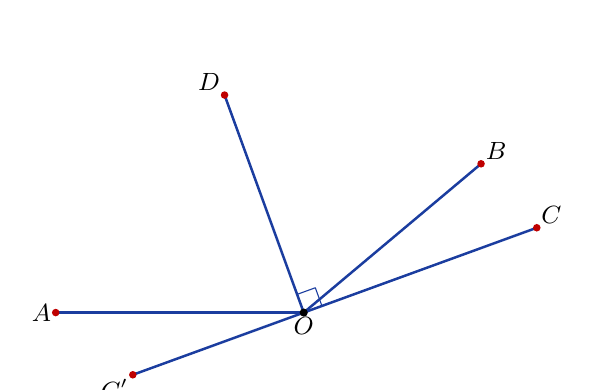
\begin{tikzpicture}[
			scale=1.05,
			line cap=round,
			line join=round,
			font=\small,
			every node/.style={inner sep=1.5pt}
		]
			\coordinate (O)  at (0,0);
			\coordinate (A)  at (180:3.0);
			\coordinate (B)  at (40:2.8);
			\coordinate (C)  at (20:3.0);
			\coordinate (D)  at (110:2.8);
			\coordinate (Cp) at (200:2.2);

			\draw[mauChuDao,line width=0.9pt] (O)--(A);
			\draw[mauChuDao,line width=0.9pt] (O)--(B);
			\draw[mauChuDao,line width=0.9pt] (Cp)--(O)--(C);
			\draw[mauChuDao,line width=0.9pt] (O)--(D);
			\pic[draw=mauChuDao,angle radius=7pt] {right angle=D--O--C};

			\fill (O) circle (1.4pt);
			\node[below] at (O) {$O$};
			\node[left] at (A) {$A$};
			\node[above right] at (B) {$B$};
			\node[above right] at (C) {$C$};
			\node[above left] at (D) {$D$};
			\node[below left] at (Cp) {$C'$};

			\foreach \P in {A,B,C,D,Cp}{
				\fill[red!75!black] (\P) circle (1.3pt);
			}
		\end{tikzpicture}
	\end{center}
\end{bt}

\begin{bt}
	Cho góc tù $\widehat{MOB}$. Vẽ tia $OC$ nằm trong góc đó. Biết
	$\widehat{MOC}+\widehat{MOB}=180^\circ$. Vẽ tia $ON$ là tia phân giác
	của $\widehat{BOC}$. Chứng minh rằng:
	
	\begin{enumerate}[label=\alph*)]
		\item $\widehat{BOC}=180^\circ-2\widehat{MOC}$.
		
		\item $OM\perp ON$.
	\end{enumerate}
\end{bt}

\subsection{Dạng 5. Bài tập tổng hợp}

\begin{bt}
	Vẽ hai góc kề bù $\widehat{xOy}$ và $\widehat{yOx'}$, biết
	$\widehat{xOy}=70^\circ$. Gọi $Ot$ và $Ot'$ lần lượt là các tia phân giác
	của $\widehat{xOy}$ và $\widehat{x'Oy}$.
	
	\begin{enumerate}[label=\alph*)]
		\item Tính $\widehat{yOx'}$ và $\widehat{xOt'}$.
		
		\item Tính $\widehat{tOt'}$. Từ đó cho biết hai tia $Ot$ và $Ot'$ có
		vuông góc với nhau không.
	\end{enumerate}
\end{bt}

\begin{bt}
	Cho hai đường thẳng $xx'$ và $yy'$ cắt nhau tại $O$, biết
	$\widehat{xOy}=40^\circ$. Các tia $Om$ và $On$ lần lượt là tia phân giác
	của $\widehat{xOy}$ và $\widehat{x'Oy'}$.
	
	\begin{enumerate}[label=\alph*)]
		\item Tính số đo các góc $\widehat{xOy'}$, $\widehat{x'Oy}$ và
		$\widehat{x'Oy'}$.
		
		\item Chứng minh $Om$ và $On$ là hai tia đối nhau.
	\end{enumerate}
\end{bt}

\begin{bt}
	Cho $\widehat{AOB}=150^\circ$. Về phía ngoài của $\widehat{AOB}$, vẽ
	hai tia $OC$ và $OD$ sao cho $OA\perp OC$ và $OB\perp OD$. Gọi $Ox$ là
	tia phân giác của $\widehat{AOB}$, $Oy$ là tia đối của tia $Ox$.
	
	\begin{enumerate}[label=\alph*)]
		\item Chứng minh $Oy$ là tia phân giác của $\widehat{COD}$.
		
		\item So sánh $\widehat{xOC}$ và $\widehat{yOB}$.
	\end{enumerate}

	\begin{flushright}
		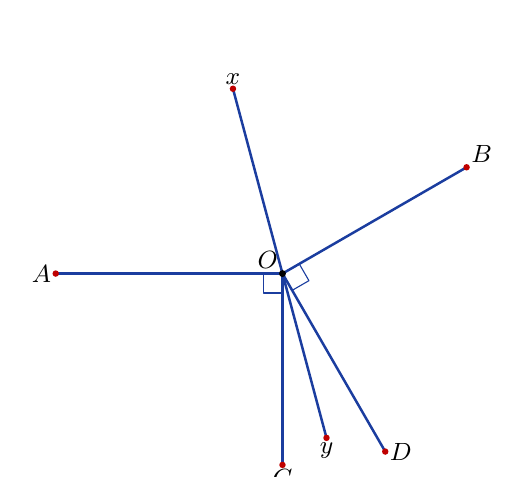
\begin{tikzpicture}[
			scale=0.9,
			line cap=round,
			line join=round,
			font=\small,
			every node/.style={inner sep=1.5pt}
		]
			\coordinate (O) at (0,0);
			\coordinate (A) at (180:3.2);
			\coordinate (B) at (30:3.0);
			\coordinate (C) at (270:2.7);
			\coordinate (D) at (300:2.9);
			\coordinate (X) at (105:2.7);
			\coordinate (Y) at (285:2.4);

			\draw[mauChuDao,line width=0.9pt] (O)--(A);
			\draw[mauChuDao,line width=0.9pt] (O)--(B);
			\draw[mauChuDao,line width=0.9pt] (O)--(C);
			\draw[mauChuDao,line width=0.9pt] (O)--(D);
			\draw[mauChuDao,line width=0.9pt] (O)--(X);
			\draw[mauChuDao,line width=0.9pt] (O)--(Y);

			\pic[draw=mauChuDao,angle radius=7pt] {right angle=A--O--C};
			\pic[draw=mauChuDao,angle radius=7pt] {right angle=B--O--D};

			\fill (O) circle (1.4pt);
			\node[above left] at (O) {$O$};
			\node[left] at (A) {$A$};
			\node[above right] at (B) {$B$};
			\node[below] at (C) {$C$};
			\node[right] at (D) {$D$};
			\node[above] at (X) {$x$};
			\node[below] at (Y) {$y$};

			\foreach \P in {A,B,C,D,X,Y}{
				\fill[red!75!black] (\P) circle (1.3pt);
			}
		\end{tikzpicture}
	\end{flushright}
\end{bt}
  

	\dang{HAI ĐƯỜNG THẲNG SONG SONG}
	\noindent
\subsection{Dạng 1. Xác định cặp góc so le trong, cặp góc đồng vị. Tính số đo góc}

\begin{bt}
	Cho hình vẽ dưới đây, trong đó hai đường thẳng $m$ và $n$ bị cắt bởi
	đường thẳng $p$ lần lượt tại $S$ và $R$.
	
	\begin{enumerate}[label=\alph*)]
		\item Kể tên các cặp góc so le trong, các cặp góc đồng vị và các cặp
		góc trong cùng phía.
		
		\item Tính số đo các góc còn lại, biết
		$\widehat{R_4}=\widehat{S_2}=120^\circ$.
	\end{enumerate}

    \begin{center}
        \begin{tikzpicture}[
            scale=1.15,
            line cap=round,
            line join=round,
            font=\small,
            every node/.style={inner sep=1.2pt}
        ]
            %--------------------------------
            % Hai giao điểm
            %--------------------------------
            \coordinate (S) at (0,1.1);
            \coordinate (R) at (1.27,-1.1);

            %--------------------------------
            % Hai đường thẳng song song m, n
            %--------------------------------
            \draw[mauChuDao,line width=0.9pt]
                (-2.3,1.1)--(2.3,1.1)
                node[right] {$m$};

            \draw[mauChuDao,line width=0.9pt]
                (-0.8,-1.1)--(3.8,-1.1)
                node[right] {$n$};

            % Ký hiệu m // n nếu muốn
            % \node at (-1.6,0.85) {$\parallel$};

            %--------------------------------
            % Đường cắt p
            %--------------------------------
            \draw[mauChuDao,line width=0.9pt]
                ($(S)+(120:1.25)$)
                --
                ($(R)+(-60:1.25)$);

            \node[above left] at ($(S)+(120:1.20)$) {$p$};

            %--------------------------------
            % Hai giao điểm
            %--------------------------------
            \fill[red!75!black] (S) circle (1.5pt);
            \fill[red!75!black] (R) circle (1.5pt);

            \node[font=\bfseries]
                at ($(S)+(90:0.72)$) {$S$};

            \node[font=\bfseries]
                at ($(R)+(270:0.72)$) {$R$};

            %--------------------------------
            % Bốn góc tại S
            %--------------------------------
            \node at ($(S)+(150:0.50)$) {$1$};
            \node at ($(S)+(60:0.50)$)  {$2$};
            \node at ($(S)+(330:0.50)$) {$3$};
            \node at ($(S)+(240:0.50)$) {$4$};

            %--------------------------------
            % Bốn góc tại R
            %--------------------------------
            \node at ($(R)+(150:0.50)$) {$1$};
            \node at ($(R)+(60:0.50)$)  {$2$};
            \node at ($(R)+(330:0.50)$) {$3$};
            \node at ($(R)+(240:0.50)$) {$4$};

            %--------------------------------
            % Đánh dấu hai góc bằng nhau
            % Ví dụ: góc S_2 và R_4
            %--------------------------------
            \draw[mauChuDao,line width=1pt]
                ($(S)+(0:0.31)$)
                arc[start angle=0,end angle=120,radius=0.31];

            \draw[mauChuDao,line width=1pt]
                ($(R)+(180:0.31)$)
                arc[start angle=180,end angle=300,radius=0.31];

        \end{tikzpicture}
    \end{center}
\end{bt}

\begin{bt}
	Cho hình vẽ dưới đây, biết $a\parallel b$ và
	$\widehat{M_1}-\widehat{N_2}=50^\circ$. Tính $\widehat{M_2}$ và
	$\widehat{N_2}$.

	\begin{center}
		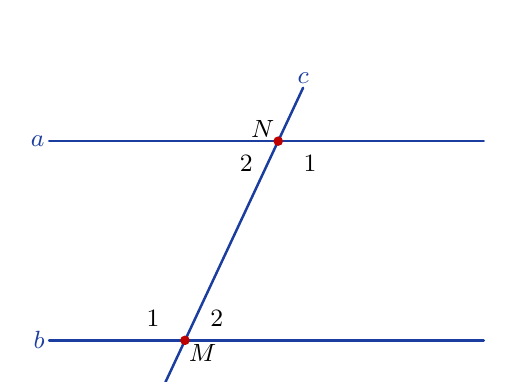
\begin{tikzpicture}[
			scale=1.15,
			line cap=round,
			line join=round,
			font=\small,
			every node/.style={inner sep=1.2pt}
		]
			\coordinate (M) at (0,-1);
			\coordinate (N) at (1.03,1.2);

			% Hai đường thẳng song song và cát tuyến c
			\draw[mauChuDao,line width=0.9pt]
				(-1.5,1.2) node[left] {$a$}--(3.3,1.2);
			\draw[mauChuDao,line width=0.9pt]
				(-1.5,-1) node[left] {$b$}--(3.3,-1);
			\draw[mauChuDao,line width=0.9pt]
				($(M)+(245:0.65)$)--($(N)+(65:0.65)$)
				node[above] {$c$};

			% Hai giao điểm
			\fill[red!75!black] (M) circle (1.5pt);
			\fill[red!75!black] (N) circle (1.5pt);
			\node[below right] at (M) {$M$};
			\node[above left] at (N) {$N$};

			% Các góc M_1, M_2, N_1, N_2
			\node at ($(M)+(145:0.43)$) {$1$};
			\node at ($(M)+(35:0.43)$) {$2$};
			\node at ($(N)+(215:0.43)$) {$2$};
			\node at ($(N)+(325:0.43)$) {$1$};
		\end{tikzpicture}
	\end{center}
\end{bt}

\begin{bt}
	Cho hình vẽ dưới đây, biết $a\parallel b$. Tính số đo $x$ và $y$.

	\begin{center}
		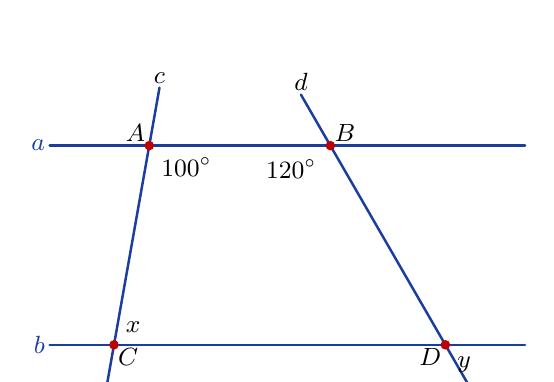
\begin{tikzpicture}[
			scale=1.15,
			line cap=round,
			line join=round,
			font=\small,
			every node/.style={inner sep=1.3pt}
		]
			\coordinate (A) at (0,1.2);
			\coordinate (B) at (2.0,1.2);
			\coordinate (C) at (-0.39,-1.0);
			\coordinate (D) at (3.27,-1.0);

			% Hai đường thẳng song song a và b
			\draw[mauChuDao,line width=0.9pt]
				(-1.1,1.2) node[left] {$a$}--(4.15,1.2);
			\draw[mauChuDao,line width=0.9pt]
				(-1.1,-1.0) node[left] {$b$}--(4.15,-1.0);

			% Hai cát tuyến c và d
			\draw[mauChuDao,line width=0.9pt]
				($(C)+(260:0.55)$)--($(A)+(80:0.65)$);
			\draw[mauChuDao,line width=0.9pt]
				($(B)+(120:0.65)$)--($(D)+(300:0.55)$);

			% Các giao điểm
			\foreach \P in {A,B,C,D}{
				\fill[red!75!black] (\P) circle (1.5pt);
			}

			% Tên điểm và tên hai cát tuyến
			\node[above left] at (A) {$A$};
			\node[above right] at (B) {$B$};
			\node[below right] at (C) {$C$};
			\node[below left] at (D) {$D$};
			\node[above] at ($(A)+(80:0.65)$) {$c$};
			\node[above] at ($(B)+(120:0.65)$) {$d$};

			% Số đo góc và các góc cần tìm
			\node[below right=4pt] at (A) {$100^\circ$};
			\node[below left=5pt] at (B) {$120^\circ$};
			\node[above right=4pt] at (C) {$x$};
			\node[below right=4pt] at (D) {$y$};
		\end{tikzpicture}
	\end{center}
\end{bt}

\subsection{Dạng 2. Chứng minh song song và tính góc}
\begin{bt}
	Cho hình vẽ dưới đây. Hai đường thẳng $PQ$ và $NO$ có song song với nhau
	không? Tại sao?


    \begin{center}
        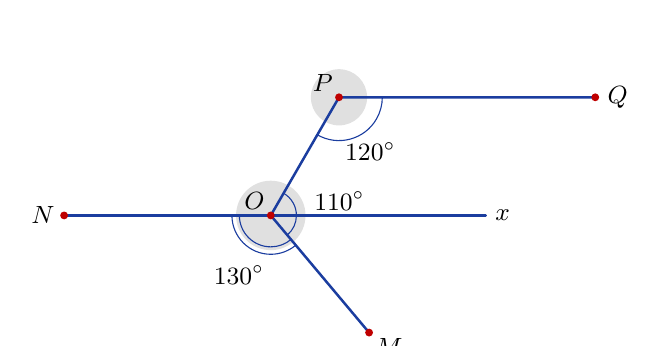
\begin{tikzpicture}[
            scale=1.05,
            line cap=round,
            line join=round,
            font=\small,
            every node/.style={inner sep=1.3pt}
        ]
            % Các tọa độ
            \coordinate (O) at (0,0);
            \coordinate (N) at (-2.5,0);
            \coordinate (X) at (2.6,0);
            \coordinate (P) at ($(O)+(60:1.65)$);
            \coordinate (Q) at ($(P)+(3.1,0)$);

            % Sửa hướng OM thành 310 độ
            \coordinate (M) at ($(O)+(310:1.85)$);

            % Hai vùng tô xám
            \fill[gray!45,opacity=0.55] (P) circle (0.34);
            \fill[gray!45,opacity=0.55] (O) circle (0.42);

            % Các đường và tia
            \draw[mauChuDao,line width=0.9pt] (P)--(Q);
            \draw[mauChuDao,line width=0.9pt] (N)--(X);
            \draw[mauChuDao,line width=0.9pt] (P)--(O)--(M);

            % Góc OPQ = 120 độ
            \pic[
                draw=mauChuDao,
                "$120^\circ$",
                angle radius=5.5mm,
                angle eccentricity=1.45
            ] {angle=O--P--Q};

            % Góc POM = 110 độ
            \draw[mauChuDao]
                ($(O)+(60:0.31)$)
                arc[start angle=60,end angle=-50,radius=0.31];

            \node[fill=white,inner sep=1pt]
                at ($(O)+(12:0.85)$) {$110^\circ$};

            % Góc NOM = 130 độ
            \draw[mauChuDao]
                ($(O)+(180:0.38)$)
                arc[start angle=180,end angle=310,radius=0.38];

            \draw[mauChuDao]
                ($(O)+(180:0.47)$)
                arc[start angle=180,end angle=310,radius=0.47];

            \node at ($(O)+(242:0.82)$) {$130^\circ$};

            % Các điểm và nhãn
            \foreach \Pnt in {N,P,O,Q,M}{
                \fill[red!75!black] (\Pnt) circle (1.35pt);
            }

            \node[above left=1pt] at (P) {$P$};
            \node[above left=1pt] at (O) {$O$};
            \node[left=2pt] at (N) {$N$};
            \node[right=3pt] at (Q) {$Q$};
            \node[right=2pt] at (X) {$x$};
            \node[below right=1pt] at (M) {$M$};

        \end{tikzpicture}
    \end{center}

\end{bt}
\begin{bt}
	Cho đoạn thẳng $AB$. Trên cùng một nửa mặt phẳng có bờ là đường thẳng
	$AB$, vẽ các tia $Ax$, $By$ sao cho
	$\widehat{ABy}=\alpha$ và $\widehat{xAB}=\dfrac{7}{2}\alpha$.
	Tính $\alpha$ để $Ax\parallel By$.
\end{bt}

\begin{bt}
	Theo hình vẽ, cho $\widehat{xOy}=70^\circ$ 
	$(\widehat{O_1}=70^\circ)$, $\widehat{A_1}=110^\circ$ và
	$\widehat{B_2}=110^\circ$. Hãy chứng minh:
	\begin{enumerate}[label=\alph*)]
		\item $a\parallel Ox$;
		\item $b\parallel Oy$.
	\end{enumerate}

    \begin{center}
        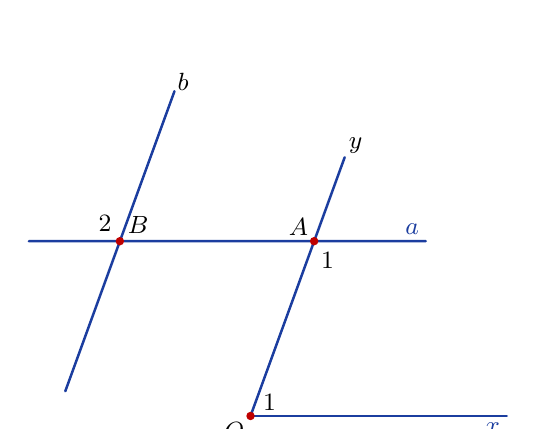
\begin{tikzpicture}[
            scale=1.05,
            line cap=round,
            line join=round,
            font=\small,
            every node/.style={inner sep=1.3pt}
        ]
            \coordinate (O) at (0,0);
            \coordinate (X) at (3.1,0);
            \coordinate (A) at ($(O)+(70:2.25)$);
            \coordinate (B) at ($(A)+(-2.35,0)$);

            % Tạo điểm Y trên tia Oy (kéo dài hơn A)
            \coordinate (Y) at ($(O)!1.48!(A)$);

            % Hai điểm phụ để vẽ đường thẳng b song song tuyệt đối với Oy
% Hai điểm gốc theo phương Oy
            \coordinate (Bleft)  at ($(B)+(O)-(Y)$);
            \coordinate (Bright) at ($(B)+(Y)-(O)$);

            % Lấy gần B hơn để đường b ngắn lại
            \coordinate (B1) at ($(B)!0.58!(Bleft)$);
            \coordinate (B2) at ($(B)!0.58!(Bright)$);

            % Đường thẳng a và tia Ox
            \draw[mauChuDao,line width=0.9pt]
                ($(B)+(-1.1,0)$)--($(A)+(1.35,0)$)
                node[above left=1pt] {$a$};

            \draw[mauChuDao,line width=0.9pt] (O)--(X)
                node[below left=1pt] {$x$};

            % Tia Oy đi qua A
            \draw[mauChuDao,line width=0.9pt] (O)--(Y);
            \node[above right] at (Y) {$y$};

            % Đường thẳng b đi qua B và song song với Oy
            \draw[mauChuDao,line width=0.9pt] (B1)--(B2);
            \node[above right] at ($(B)!0.98!(B2)$) {$b$};

            % Các giao điểm
            \foreach \Pnt in {O,A,B}{
                \fill[red!75!black] (\Pnt) circle (1.45pt);
            }

            \node[below left=1pt] at (O) {$O$};
            \node[above left=1pt] at (A) {$A$};
            \node[above right=2pt] at (B) {$B$};

            % Ký hiệu các góc O_1, A_1 và B_2
            \node at ($(O)+(35:0.28)$) {$1$};
            \node at ($(A)+(-55:0.28)$) {$1$};
            \node at ($(B)+(130:0.28)$) {$2$};
        \end{tikzpicture}
    \end{center}

\end{bt}
\subsection{Dạng 3. Tổng hợp tính góc và chứng minh song song}
\begin{bt}
	Cho hình vẽ. Tìm trên hình các đường thẳng song song với $OC$.
	Vì sao?

	\begin{center}
		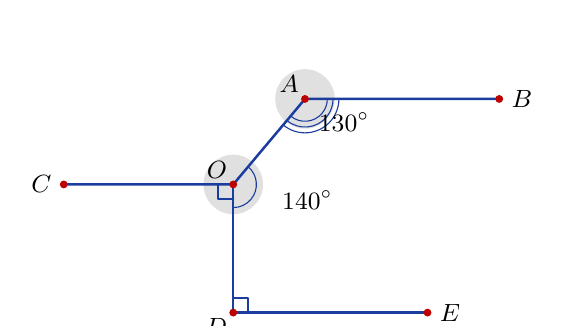
\begin{tikzpicture}[
			scale=1.05,
			line cap=round,
			line join=round,
			font=\small,
			every node/.style={inner sep=1.3pt}
		]
			\coordinate (O) at (0,0);
			\coordinate (C) at (-2.05,0);
			\coordinate (D) at (0,-1.55);
			\coordinate (E) at (2.35,-1.55);
			\coordinate (A) at ($(O)+(50:1.35)$);
			\coordinate (B) at ($(A)+(2.35,0)$);

			% Vùng tô xám quanh hai đỉnh có góc đã cho
			\fill[gray!45,opacity=0.55] (O) circle (0.36);
			\fill[gray!45,opacity=0.55] (A) circle (0.36);

			% Các đường và đoạn thẳng
			\draw[mauChuDao,line width=0.9pt] (C)--(O)--(A)--(B);
			\draw[mauChuDao,line width=0.9pt] (O)--(D)--(E);

			% Góc 140 độ tại O
			\draw[mauChuDao] ($(O)+(50:0.28)$)
				arc[start angle=50,end angle=-90,radius=0.28];
			\node[right=3pt] at ($(O)+(-23:0.48)$) {$140^\circ$};

			% Góc 130 độ tại A với các cung đồng tâm
			\draw[mauChuDao] ($(A)+(230:0.27)$)
				arc[start angle=230,end angle=360,radius=0.27];
			\draw[mauChuDao] ($(A)+(230:0.34)$)
				arc[start angle=230,end angle=360,radius=0.34];
			\draw[mauChuDao] ($(A)+(230:0.41)$)
				arc[start angle=230,end angle=360,radius=0.41];
			\node[below right=5pt] at (A) {$130^\circ$};

			% Dấu vuông: OD vuông góc OC và OD vuông góc DE
			\draw[mauChuDao,line width=0.8pt]
				($(O)+(-0.18,0)$)--($(O)+(-0.18,-0.18)$)--($(O)+(0,-0.18)$);
			\draw[mauChuDao,line width=0.8pt]
				($(D)+(0,0.18)$)--($(D)+(0.18,0.18)$)--($(D)+(0.18,0)$);

			% Các điểm và nhãn
			\foreach \Pnt in {C,O,A,B,D,E}{
				\fill[red!75!black] (\Pnt) circle (1.35pt);
			}
			\node[left=3pt] at (C) {$C$};
			\node[above left=1pt] at (O) {$O$};
			\node[above left=1pt] at (A) {$A$};
			\node[right=3pt] at (B) {$B$};
			\node[below left=1pt] at (D) {$D$};
			\node[right=3pt] at (E) {$E$};
		\end{tikzpicture}
	\end{center}
\end{bt}

\begin{bt}
	Cho hình vẽ sau. Biết
	$\widehat{AMN}=2\widehat{BMN}$ và
	$\widehat{MND}-\widehat{MNC}=60^\circ$.
	Chứng minh rằng $AB\parallel CD$.

	\begin{center}
		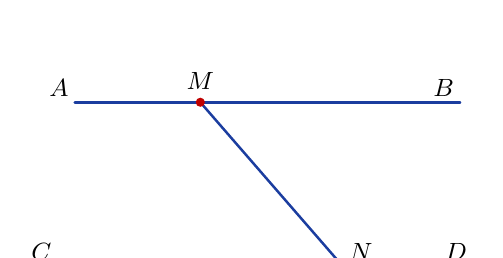
\begin{tikzpicture}[
			scale=1.1,
			line cap=round,
			line join=round,
			font=\small,
			every node/.style={inner sep=1.3pt}
		]
			\coordinate (M) at (0,1.25);
			\coordinate (N) at (1.65,-0.65);
			\coordinate (A) at (-1.45,1.25);
			\coordinate (B) at (3.0,1.25);
			\coordinate (C) at (-1.65,-0.65);
			\coordinate (D) at (3.15,-0.65);

			% Hai đường thẳng AB, CD và cát tuyến MN
			\draw[mauChuDao,line width=0.9pt] (A)--(B);
			\draw[mauChuDao,line width=0.9pt] (C)--(D);
			\draw[mauChuDao,line width=0.9pt] (M)--(N);

			% Hai giao điểm
			\fill[red!75!black] (M) circle (1.5pt);
			\fill[red!75!black] (N) circle (1.5pt);

			% Nhãn các điểm
			\node[above left=1pt] at (A) {$A$};
			\node[above=3pt] at (M) {$M$};
			\node[above left=1pt] at (B) {$B$};
			\node[above left=1pt] at (C) {$C$};
			\node[above right=1pt] at (N) {$N$};
			\node[above left=1pt] at (D) {$D$};
		\end{tikzpicture}
	\end{center}
\end{bt}

\begin{bt}
	Cho hình vẽ sau. Chứng minh rằng $AB\parallel CD$.

	\begin{center}
		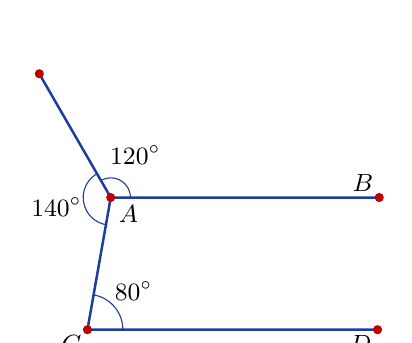
\begin{tikzpicture}[
			scale=1.1,
			line cap=round,
			line join=round,
			font=\small,
			every node/.style={inner sep=1.3pt}
		]
			\coordinate (A) at (0,0);
			\coordinate (B) at (3.1,0);
			\coordinate (P) at ($(A)+(120:1.65)$);
			\coordinate (C) at ($(A)+(260:1.55)$);
			\coordinate (D) at ($(C)+(3.35,0)$);

			% Các đoạn thẳng trong hình
			\draw[mauChuDao,line width=0.9pt] (P)--(A)--(B);
			\draw[mauChuDao,line width=0.9pt] (A)--(C)--(D);

			% Các góc đã cho tại A và C
			\pic[draw=mauChuDao,"$120^\circ$",angle radius=2.5mm,
				angle eccentricity=2.5] {angle=B--A--P};
			\pic[draw=mauChuDao,"$140^\circ$",angle radius=3.5mm,
				angle eccentricity=2] {angle=P--A--C};
			\pic[draw=mauChuDao,"$80^\circ$",angle radius=4.5mm,
				angle eccentricity=1.7] {angle=D--C--A};

			% Các điểm
			\foreach \Pnt in {P,A,B,C,D}{
				\fill[red!75!black] (\Pnt) circle (1.5pt);
			}

			% Nhãn các điểm
			\node[below right=2pt] at (A) {$A$};
			\node[above left=1pt] at (B) {$B$};
			\node[below left=1pt] at (C) {$C$};
			\node[below left=1pt] at (D) {$D$};
		\end{tikzpicture}
	\end{center}
\end{bt}


	\dang{TỪ VUÔNG GÓC ĐẾN SONG SONG – TIÊN ĐỀ Ơ-CLÍT}
	\subsection{Dạng 1. Tính số đo góc (bằng cách vẽ thêm hình)}

\begin{bt}
	Cho hình vẽ, biết $MN\parallel KJ$,
	$\widehat{NML}=46^\circ$ và $\widehat{JKL}=127^\circ$.
	Hãy tính số đo góc $\widehat{MLK}$.

	\begin{center}
		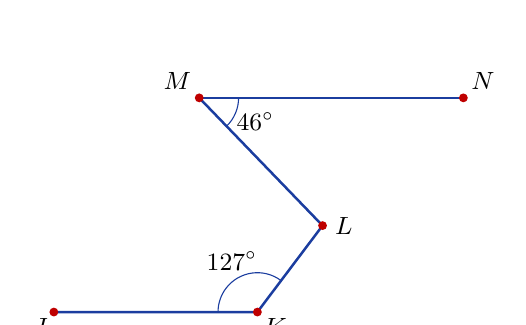
\begin{tikzpicture}[
			scale=1.1,
			line cap=round,
			line join=round,
			font=\small,
			every node/.style={inner sep=1.3pt}
		]
			\coordinate (M) at (0,1.5);
			\coordinate (N) at (3.05,1.5);
			\coordinate (L) at ($(M)+(-46:2.05)$);
			\coordinate (K) at ($(L)+(233:1.25)$);
			\coordinate (J) at ($(K)+(-2.35,0)$);

			% Hai đường thẳng song song và đường gấp MLK
			\draw[mauChuDao,line width=0.9pt] (M)--(N);
			\draw[mauChuDao,line width=0.9pt] (J)--(K);
			\draw[mauChuDao,line width=0.9pt] (M)--(L)--(K);

			% Hai góc đã biết
			\pic[draw=mauChuDao,"$46^\circ$",angle radius=5mm,
				angle eccentricity=1.55] {angle=L--M--N};
			\pic[draw=mauChuDao,"$127^\circ$",angle radius=5mm,
				angle eccentricity=1.45] {angle=L--K--J};

			% Các điểm và nhãn
			\foreach \Pnt in {M,N,L,K,J}{
				\fill[red!75!black] (\Pnt) circle (1.45pt);
			}
			\node[above left=2pt] at (M) {$M$};
			\node[above right=2pt] at (N) {$N$};
			\node[right=3pt] at (L) {$L$};
			\node[below right=1pt] at (K) {$K$};
			\node[below left=1pt] at (J) {$J$};
		\end{tikzpicture}
	\end{center}
\end{bt}

\begin{bt}
	Cho hình vẽ, biết $AB\parallel ED$,
	$\widehat{BAC}=118^\circ$ và $\widehat{CDE}=50^\circ$.
	Hãy tính số đo góc $\widehat{ACD}$.

	\begin{center}
		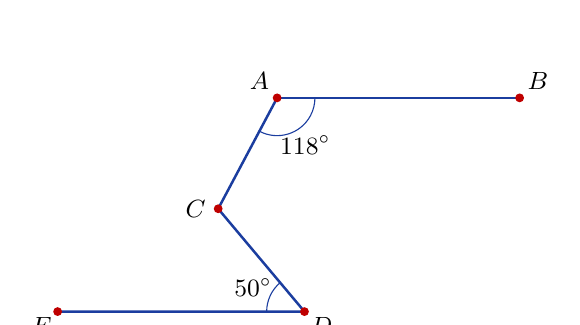
\begin{tikzpicture}[
			scale=1.1,
			line cap=round,
			line join=round,
			font=\small,
			every node/.style={inner sep=1.3pt}
		]
			\coordinate (A) at (0,1.55);
			\coordinate (B) at (2.8,1.55);
			\coordinate (C) at ($(A)+(242:1.45)$);
			\coordinate (D) at ($(C)+(310:1.55)$);
			\coordinate (E) at ($(D)+(-2.85,0)$);

			% Hai đường thẳng song song và đường gấp ACD
			\draw[mauChuDao,line width=0.9pt] (A)--(B);
			\draw[mauChuDao,line width=0.9pt] (E)--(D);
			\draw[mauChuDao,line width=0.9pt] (A)--(C)--(D);

			% Hai góc đã biết
			\pic[draw=mauChuDao,"$118^\circ$",angle radius=4.8mm,
				angle eccentricity=1.45] {angle=C--A--B};
			\pic[draw=mauChuDao,"$50^\circ$",angle radius=4.8mm,
				angle eccentricity=1.5] {angle=C--D--E};

			% Các điểm và nhãn
			\foreach \Pnt in {A,B,C,D,E}{
				\fill[red!75!black] (\Pnt) circle (1.45pt);
			}
			\node[above left=2pt] at (A) {$A$};
			\node[above right=2pt] at (B) {$B$};
			\node[left=3pt] at (C) {$C$};
			\node[below right=1pt] at (D) {$D$};
			\node[below left=1pt] at (E) {$E$};
		\end{tikzpicture}
	\end{center}
\end{bt}

\begin{bt}
	Cho hình vẽ, biết ba điểm $C,B,E$ thẳng hàng, $AB\parallel FG$,
	$\widehat{ABC}=49^\circ$ và $\widehat{EFG}=120^\circ$.
	Hãy tính số đo góc $\widehat{CEF}$.

	\begin{center}
		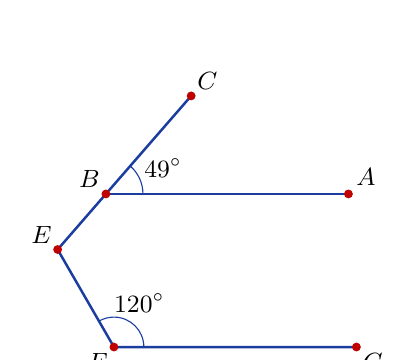
\begin{tikzpicture}[
			scale=1.1,
			line cap=round,
			line join=round,
			font=\small,
			every node/.style={inner sep=1.3pt}
		]
			\coordinate (B) at (0,0.9);
			\coordinate (A) at (2.8,0.9);
			\coordinate (C) at ($(B)+(49:1.5)$);
			\coordinate (E) at ($(B)+(229:0.85)$);
			\coordinate (F) at ($(E)+(300:1.3)$);
			\coordinate (G) at ($(F)+(2.8,0)$);

			% Hai đường thẳng song song và đường gấp CEF
			\draw[mauChuDao,line width=0.9pt] (B)--(A);
			\draw[mauChuDao,line width=0.9pt] (F)--(G);
			\draw[mauChuDao,line width=0.9pt] (C)--(B)--(E)--(F);

			% Hai góc đã biết
			\pic[draw=mauChuDao,"$49^\circ$",angle radius=4.7mm,
				angle eccentricity=1.7] {angle=A--B--C};
			\pic[draw=mauChuDao,"$120^\circ$",angle radius=3.8mm,
				angle eccentricity=1.7] {angle=G--F--E};

			% Các điểm và nhãn
			\foreach \Pnt in {A,B,C,E,F,G}{
				\fill[red!75!black] (\Pnt) circle (1.45pt);
			}
			\node[above right=2pt] at (A) {$A$};
			\node[above left=1pt] at (B) {$B$};
			\node[above right=1pt] at (C) {$C$};
			\node[above left=1pt] at (E) {$E$};
			\node[below left=1pt] at (F) {$F$};
			\node[below right=1pt] at (G) {$G$};
		\end{tikzpicture}
	\end{center}
\end{bt}

\subsection{Dạng 2. Chứng minh hai đường thẳng song song}

\begin{bt}
	Theo hình vẽ, cho
	$\widehat{xAB}+\widehat{ABC}+\widehat{BCy}=360^\circ$.
	Hãy chứng minh $Ax\parallel Cy$.

	\begin{center}
		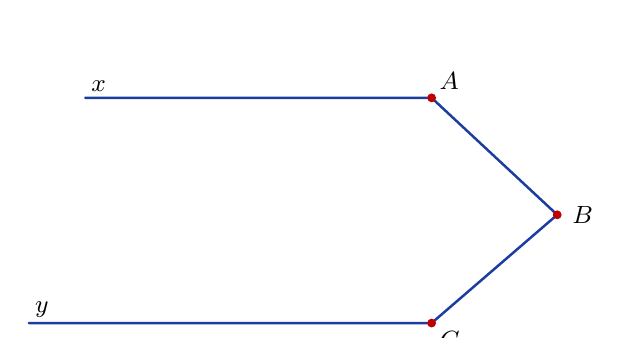
\begin{tikzpicture}[
			scale=1.1,
			line cap=round,
			line join=round,
			font=\small,
			every node/.style={inner sep=1.3pt}
		]
			\coordinate (A) at (1.3,1.35);
			\coordinate (B) at (2.75,0);
			\coordinate (C) at (1.3,-1.25);
			\coordinate (X) at (-2.7,1.35);
			\coordinate (Y) at (-3.35,-1.25);

			% Hai tia Ax, Cy và đường gấp ABC
			\draw[mauChuDao,line width=0.9pt] (X)--(A)--(B)--(C)--(Y);

			% Các đỉnh của đường gấp
			\foreach \Pnt in {A,B,C}{
				\fill[red!75!black] (\Pnt) circle (1.45pt);
			}

			% Nhãn các điểm và tên tia
			\node[above right=2pt] at (A) {$A$};
			\node[right=4pt] at (B) {$B$};
			\node[below right=2pt] at (C) {$C$};
			\node[above right=1pt] at (X) {$x$};
			\node[above right=1pt] at (Y) {$y$};
		\end{tikzpicture}
	\end{center}
\end{bt}

\begin{bt}
	Cho hình vẽ bên. Biết $My\parallel Pt$,
	$\widehat{xMy}=60^\circ$ và $\widehat{MNz}=60^\circ$.
	\begin{enumerate}[label=\alph*)]
		\item Chứng minh $My\parallel Nz$;
		\item Chứng minh $Nz\parallel Pt$;
		\item Biết $\widehat{xNP}=85^\circ$, tính số đo góc $\widehat{NPt}$.
	\end{enumerate}

	\begin{center}
		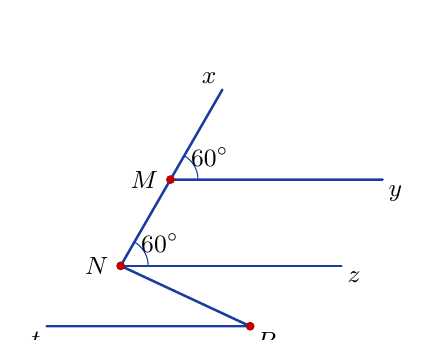
\begin{tikzpicture}[
			scale=1.1,
			line cap=round,
			line join=round,
			font=\small,
			every node/.style={inner sep=1.3pt}
		]
			\coordinate (N) at (0,0);
			\coordinate (M) at ($(N)+(60:1.15)$);
			\coordinate (X) at ($(M)+(60:1.2)$);
			\coordinate (Y) at ($(M)+(2.45,0)$);
			\coordinate (Z) at ($(N)+(2.55,0)$);
			\coordinate (P) at ($(N)+(-25:1.65)$);
			\coordinate (T) at ($(P)+(-2.35,0)$);

			% Các tia và đoạn thẳng trong hình
			\draw[mauChuDao,line width=0.9pt] (N)--(M)--(X);
			\draw[mauChuDao,line width=0.9pt] (M)--(Y);
			\draw[mauChuDao,line width=0.9pt] (N)--(Z);
			\draw[mauChuDao,line width=0.9pt] (N)--(P)--(T);

			% Hai góc 60 độ
			\pic[draw=mauChuDao,"$60^\circ$",angle radius=3.5mm,
				angle eccentricity=1.65] {angle=Y--M--X};
			\pic[draw=mauChuDao,"$60^\circ$",angle radius=3.5mm,
				angle eccentricity=1.65] {angle=Z--N--M};

			% Các điểm
			\foreach \Pnt in {M,N,P}{
				\fill[red!75!black] (\Pnt) circle (1.45pt);
			}

			% Nhãn các điểm và tên tia
			\node[left=3pt] at (M) {$M$};
			\node[left=3pt] at (N) {$N$};
			\node[below right=1pt] at (P) {$P$};
			\node[above left=1pt] at (X) {$x$};
			\node[below right=1pt] at (Y) {$y$};
			\node[below right=1pt] at (Z) {$z$};
			\node[below left=1pt] at (T) {$t$};
		\end{tikzpicture}
	\end{center}
\end{bt}

\begin{bt}
	Cho hình vẽ sau, biết $HD\parallel GE$ và $GE\parallel IF$.
	\begin{enumerate}[label=\alph*)]
		\item Chứng minh $HD\parallel IF$.
		\item Cho biết $\widehat{HAB}=65^\circ$. Tìm số đo $x$ của góc
		$\widehat{ABE}$ và số đo $y$ của góc $\widehat{BCI}$.
	\end{enumerate}

	\begin{center}
		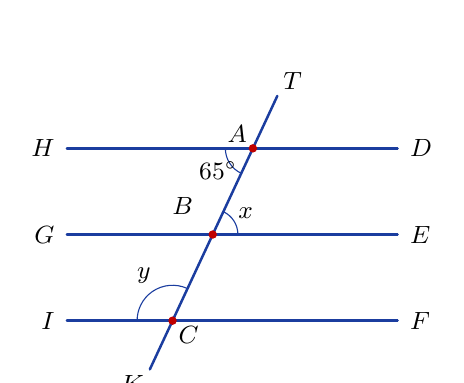
\begin{tikzpicture}[
			scale=1.05,
			line cap=round,
			line join=round,
			font=\small,
			every node/.style={inner sep=1.3pt}
		]
			\coordinate (A) at (0,1.9);
			\coordinate (B) at ($(A)+(245:1.15)$);
			\coordinate (C) at ($(B)+(245:1.15)$);
			\coordinate (T) at ($(A)+(65:0.7)$);
			\coordinate (K) at ($(C)+(245:0.65)$);

			\coordinate (H) at (-2.25,1.9);
			\coordinate (D) at (1.75,1.9);
			\coordinate (G) at (-2.25,{1.9-1.15*sin(65)});
			\coordinate (E) at (1.75,{1.9-1.15*sin(65)});
			\coordinate (I) at (-2.25,{1.9-2.3*sin(65)});
			\coordinate (F) at (1.75,{1.9-2.3*sin(65)});

			% Ba đường thẳng song song và cát tuyến
			\draw[mauChuDao,line width=0.9pt] (H)--(D);
			\draw[mauChuDao,line width=0.9pt] (G)--(E);
			\draw[mauChuDao,line width=0.9pt] (I)--(F);
			\draw[mauChuDao,line width=0.9pt] (K)--(T);

			% Góc HAB và hai góc cần tìm x, y
			\pic[draw=mauChuDao,"$65^\circ$",angle radius=3.5mm,
				angle eccentricity=1.5] {angle=H--A--B};
			\pic[draw=mauChuDao,"$x$",angle radius=3.2mm,
				angle eccentricity=1.55] {angle=E--B--A};
			\pic[draw=mauChuDao,"$y$",angle radius=4.5mm,
				angle eccentricity=1.5] {angle=B--C--I};

			% Các giao điểm
			\foreach \Pnt in {A,B,C}{
				\fill[red!75!black] (\Pnt) circle (1.45pt);
			}

			% Nhãn các điểm
			\node[left=3pt] at (H) {$H$};
			\node[right=3pt] at (D) {$D$};
			\node[left=3pt] at (G) {$G$};
			\node[right=3pt] at (E) {$E$};
			\node[left=3pt] at (I) {$I$};
			\node[right=3pt] at (F) {$F$};
			\node[above left=1pt] at (A) {$A$};
			\node[above left=8pt] at (B) {$B$};
			\node[below right=1pt] at (C) {$C$};
			\node[above right=1pt] at (T) {$T$};
			\node[below left=1pt] at (K) {$K$};
		\end{tikzpicture}
	\end{center}
\end{bt}
\begin{bt}
	Cho hình vẽ, biết $\widehat{A_2}=\widehat{M_1}$ và
	$\widehat{A_1}=\widehat{N_2}$.
	\begin{enumerate}[label=\alph*)]
		\item Cho biết $\widehat{A_2}$ và $\widehat{M_1}$ là hai góc ở vị trí
		như thế nào.
		\item Hai góc $\widehat{A_1}$ và $\widehat{N_2}$ là hai góc gì?
		\item Chứng minh $MD\parallel AH$.
		\item Chứng minh $NE\parallel MD$.
	\end{enumerate}

	\begin{center}
		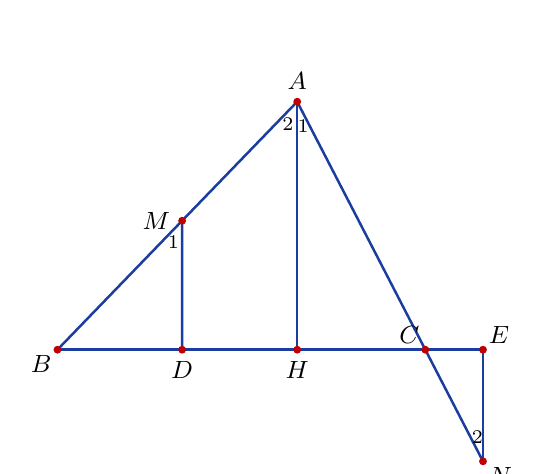
\begin{tikzpicture}[
			scale=1.05,
			line cap=round,
			line join=round,
			font=\small,
			every node/.style={inner sep=1.2pt}
		]
			\coordinate (A) at (0,3.0);
			\coordinate (H) at (0,0);
			\coordinate (B) at (-2.9,0);
			\coordinate (C) at (1.55,0);
			\coordinate (N) at (2.2475,-1.35);
			\coordinate (E) at (2.2475,0);
			\coordinate (M) at ($(B)!0.52!(A)$);
			\coordinate (D) at ($(M |- H)$);

			% Đường đáy và các đường trong hình
			\draw[mauChuDao,line width=0.9pt] (B)--(E);
			\draw[mauChuDao,line width=0.9pt] (B)--(A)--(C)--(N);
			\draw[mauChuDao,line width=0.9pt] (A)--(H);
			\draw[mauChuDao,line width=0.9pt] (M)--(D);
			\draw[mauChuDao,line width=0.9pt] (N)--(E);

			% Ký hiệu các góc A_1, A_2, M_1 và N_2
			\node[font=\scriptsize] at ($(A)+(-76:0.30)$) {$1$};
			\node[font=\scriptsize] at ($(A)+(-112:0.30)$) {$2$};
			\node[font=\scriptsize] at ($(M)+(-112:0.28)$) {$1$};
			\node[font=\scriptsize] at ($(N)+(103:0.30)$) {$2$};

			\foreach \Pnt in {A,B,C,D,E,H,M,N}{
				\fill[red!75!black] (\Pnt) circle (1.35pt);
			}
			\node[above=3pt] at (A) {$A$};
			\node[below left=1pt] at (B) {$B$};
			\node[above left=1pt] at (C) {$C$};
			\node[below=3pt] at (D) {$D$};
			\node[above right=1pt] at (E) {$E$};
			\node[below=3pt] at (H) {$H$};
			\node[left=3pt] at (M) {$M$};
			\node[below right=1pt] at (N) {$N$};
		\end{tikzpicture}
	\end{center}
\end{bt}

\subsection{Dạng 3. Chứng minh song song do cùng vuông góc}

\begin{bt}
	Cho góc nhọn $\widehat{AOB}$. Từ $M$ trên tia $OA$ vẽ
	$MN\perp OB$ $(N\in OB)$; từ $N$ vẽ $NP\perp OA$ $(P\in OA)$;
	từ $P$ vẽ $PQ\perp OB$ $(Q\in OB)$; từ $Q$ vẽ
	$QR\perp OA$ $(R\in OA)$.
	\begin{enumerate}[label=\alph*)]
		\item Chứng minh $MN\parallel PQ$ và $NP\parallel QR$.
		\item Trong hình vẽ, xác định tất cả các góc có số đo bằng
		$\widehat{PMN}$ và tất cả các góc có số đo bằng $\widehat{MNP}$.
	\end{enumerate}

	\begin{center}
		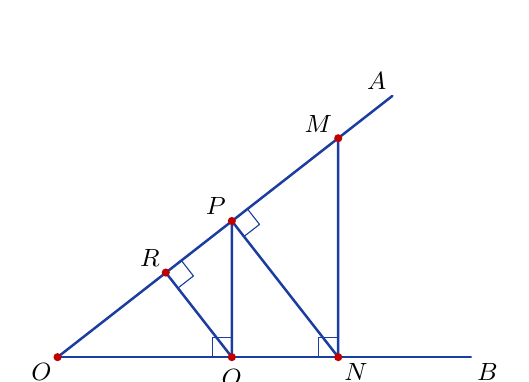
\begin{tikzpicture}[
			scale=1.05,
			line cap=round,
			line join=round,
			font=\small,
			every node/.style={inner sep=1.3pt}
		]
			\coordinate (O) at (0,0);
			\coordinate (B) at (5.0,0);
			\coordinate (A) at (4.05,3.16);
			\coordinate (M) at (3.395,2.648);
			\coordinate (N) at (3.395,0);
			\coordinate (P) at (2.108,1.647);
			\coordinate (Q) at (2.108,0);
			\coordinate (R) at (1.309,1.023);

			% Hai tia của góc AOB
			\draw[mauChuDao,line width=0.9pt] (O)--(A);
			\draw[mauChuDao,line width=0.9pt] (O)--(B);

			% Các đoạn vuông góc liên tiếp
			\draw[mauChuDao,line width=0.9pt] (M)--(N)--(P)--(Q)--(R);

			% Dấu vuông góc tại N, P, Q và R
			\pic[draw=mauChuDao,angle radius=2.5mm]
				{right angle=M--N--O};
			\pic[draw=mauChuDao,angle radius=2.5mm]
				{right angle=M--P--N};
			\pic[draw=mauChuDao,angle radius=2.5mm]
				{right angle=P--Q--O};
			\pic[draw=mauChuDao,angle radius=2.5mm]
				{right angle=P--R--Q};

			% Các điểm
			\foreach \Pnt in {O,M,N,P,Q,R}{
				\fill[red!75!black] (\Pnt) circle (1.4pt);
			}

			% Nhãn các điểm
			\node[below left=1pt] at (O) {$O$};
			\node[above left=1pt] at (A) {$A$};
			\node[below right=1pt] at (B) {$B$};
			\node[above left=1pt] at (M) {$M$};
			\node[below right=1pt] at (N) {$N$};
			\node[above left=1pt] at (P) {$P$};
			\node[below=3pt] at (Q) {$Q$};
			\node[above left=1pt] at (R) {$R$};
		\end{tikzpicture}
	\end{center}
\end{bt}

\subsection{Dạng 4. Chứng minh vuông góc từ song song}

\begin{bt}
	Cho hình vẽ. Biết $a\parallel b$, $b\perp c$ và tia $Ad$ là tia
	phân giác của góc $\widehat{cAx}$, trong đó tia $Ax$ nằm trên đường
	thẳng $a$.
	\begin{enumerate}[label=\alph*)]
		\item Chứng minh $a\perp c$.
		\item Tính số đo góc $\widehat{cAd}$.
	\end{enumerate}

	\begin{center}
		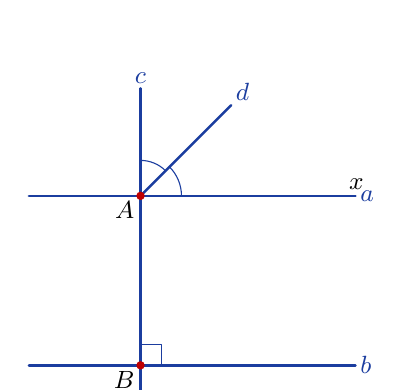
\begin{tikzpicture}[
			scale=1.05,
			line cap=round,
			line join=round,
			font=\small,
			every node/.style={inner sep=1.3pt}
		]
			\coordinate (A) at (0,1.05);
			\coordinate (B) at (0,-1.0);
			\coordinate (X) at (2.45,1.05);
			\coordinate (D) at ($(A)+(45:1.55)$);
			\coordinate (BR) at (1,-1.0);
			\coordinate (CT) at (0,2.05);

			% Hai đường thẳng song song a, b và đường thẳng c
			\draw[mauChuDao,line width=0.9pt]
				(-1.35,1.05)--(2.6,1.05) node[right] {$a$};
			\draw[mauChuDao,line width=0.9pt]
				(-1.35,-1.0)--(2.6,-1.0) node[right] {$b$};
			\draw[mauChuDao,line width=0.9pt]
				(0,-1.45)--(0,2.35) node[above] {$c$};
			\draw[mauChuDao,line width=0.9pt] (A)--(D)
				node[above right] {$d$};

			% Dấu vuông tại B và hai cung bằng nhau tại A
			\pic[draw=mauChuDao,angle radius=2.7mm]
				{right angle=A--B--BR};
			\pic[draw=mauChuDao,angle radius=4.5mm]
				{angle=D--A--CT};
			\pic[draw=mauChuDao,angle radius=5.2mm]
				{angle=X--A--D};

			\fill[red!75!black] (A) circle (1.45pt);
			\fill[red!75!black] (B) circle (1.45pt);
			\node[below left=1pt] at (A) {$A$};
			\node[below left=1pt] at (B) {$B$};
			\node[above right=1pt] at (X) {$x$};
		\end{tikzpicture}
	\end{center}
\end{bt}

\begin{bt}
	Cho hình vẽ. Đường thẳng $c$ cắt $m$ tại $C$ và cắt $n$ tại $D$.
	Biết $\widehat{C_1}=\widehat{D_1}$ và $AB\perp m$.
	\begin{enumerate}[label=\alph*)]
		\item Chứng minh $m\parallel n$.
		\item Chứng minh $AB\perp n$.
	\end{enumerate}

	\begin{center}
		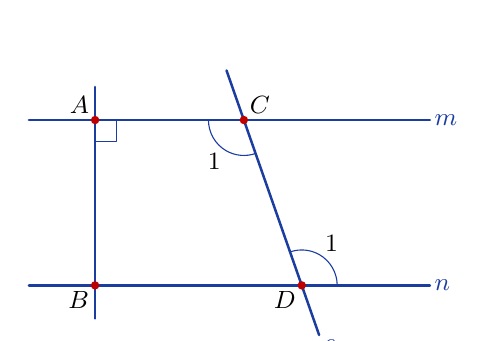
\begin{tikzpicture}[
			scale=1.05,
			line cap=round,
			line join=round,
			font=\small,
			every node/.style={inner sep=1.3pt}
		]
			\coordinate (A) at (-1.45,1.0);
			\coordinate (B) at (-1.45,-1.0);
			\coordinate (C) at (0.35,1.0);
			\coordinate (D) at (1.05,-1.0);
			\coordinate (AR) at (-0.45,1.0);
			\coordinate (CL) at (-0.65,1.0);
			\coordinate (DR) at (2.05,-1.0);

			% Hai đường m, n; đường AB và cát tuyến c
			\draw[mauChuDao,line width=0.9pt]
				(-2.25,1.0)--(2.6,1.0) node[right] {$m$};
			\draw[mauChuDao,line width=0.9pt]
				(-2.25,-1.0)--(2.6,-1.0) node[right] {$n$};
			\draw[mauChuDao,line width=0.9pt] (-1.45,-1.4)--(-1.45,1.4);
			\draw[mauChuDao,line width=0.9pt]
				($(C)!-0.3!(D)$)--($(C)!1.3!(D)$) node[below right] {$c$};

			% Dấu vuông tại A
			\pic[draw=mauChuDao,angle radius=2.7mm]
				{right angle=B--A--AR};

			% Hai góc so le trong bằng nhau
			\pic[draw=mauChuDao,"$1$",angle radius=4.5mm,
				angle eccentricity=1.45]
				{angle=CL--C--D};
			\pic[draw=mauChuDao,"$1$",angle radius=4.5mm,
				angle eccentricity=1.45]
				{angle=DR--D--C};

			% Các giao điểm và nhãn
			\foreach \Pnt in {A,B,C,D}{
				\fill[red!75!black] (\Pnt) circle (1.45pt);
			}
			\node[above left=1pt] at (A) {$A$};
			\node[below left=1pt] at (B) {$B$};
			\node[above right=1pt] at (C) {$C$};
			\node[below left=1pt] at (D) {$D$};
		\end{tikzpicture}
	\end{center}
\end{bt}

\subsection{Dạng 5. Chứng minh thẳng hàng}

\begin{bt}
	Cho hình vẽ bên, biết $Ax\parallel Dy$,
	$\widehat{BCD}=135^\circ$, $AE\perp Ax$ và $CD\perp Dy$.
	\begin{enumerate}[label=\arabic*)]
		\item Đường thẳng $AE$ có vuông góc với $Dy$ không? Vì sao?
		\item Chứng minh $DC\parallel AE$.
		\item Vẽ tia phân giác $Dt$ của góc $\widehat{CDy}$; tia $Dt$ cắt
		đường thẳng $AE$ tại $F$. Tính $\widehat{EDF}$ và $\widehat{DFB}$.
		\item Trên nửa mặt phẳng có bờ là đường thẳng $AB$ không chứa điểm
		$C$, vẽ tia $Bz$ sao cho $\widehat{ABz}=45^\circ$. Tia $Bz$ cắt
		tia $Ax$ tại $M$. Chứng minh ba điểm $B,C,M$ thẳng hàng.
	\end{enumerate}

	\begin{center}
		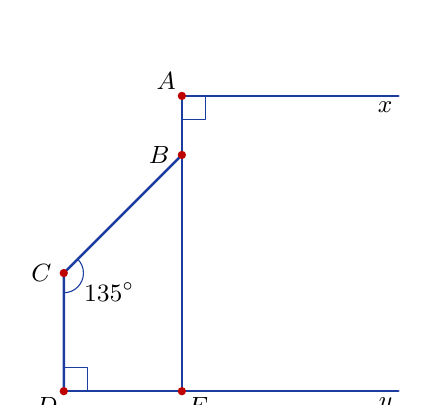
\begin{tikzpicture}[
			scale=1.0,
			line cap=round,
			line join=round,
			font=\small,
			every node/.style={inner sep=1.3pt}
		]
			\coordinate (D) at (0,0);
			\coordinate (C) at (0,1.5);
			\coordinate (E) at (1.5,0);
			\coordinate (B) at (1.5,3.0);
			\coordinate (A) at (1.5,3.75);
			\coordinate (X) at (4.25,3.75);
			\coordinate (Y) at (4.25,0);
			\coordinate (ER) at (2.5,0);
			\coordinate (AD) at (1.5,2.75);

			% Hai tia song song Ax, Dy và các đoạn AE, CD, CB
			\draw[mauChuDao,line width=0.9pt] (A)--(X);
			\draw[mauChuDao,line width=0.9pt] (D)--(Y);
			\draw[mauChuDao,line width=0.9pt] (A)--(E);
			\draw[mauChuDao,line width=0.9pt] (D)--(C)--(B);

			% Hai dấu vuông góc tại A và D
			\pic[draw=mauChuDao,angle radius=3mm]
				{right angle=AD--A--X};
			\pic[draw=mauChuDao,angle radius=3mm]
				{right angle=C--D--ER};

			% Góc BCD bằng 135 độ
			\pic[draw=mauChuDao,"$135^\circ$",angle radius=2.5mm,
				angle eccentricity=2.5] {angle=D--C--B};

			% Các điểm
			\foreach \Pnt in {A,B,C,D,E}{
				\fill[red!75!black] (\Pnt) circle (1.5pt);
			}

			% Nhãn các điểm và tên tia
			\node[above left=1pt] at (A) {$A$};
			\node[left=3pt] at (B) {$B$};
			\node[left=3pt] at (C) {$C$};
			\node[below left=1pt] at (D) {$D$};
			\node[below right=1pt] at (E) {$E$};
			\node[below left=1pt] at (X) {$x$};
			\node[below left=1pt] at (Y) {$y$};
		\end{tikzpicture}
	\end{center}
\end{bt}







\end{document}